\documentclass{article}
\usepackage[utf8]{inputenc}
\usepackage[spanish]{babel}
\usepackage{listings}
\usepackage{graphicx}
\graphicspath{ {Images/} }
\usepackage{cite}

\begin{document}

\begin{titlepage}
    \begin{center}
        \vspace*{1cm}
            
        \Huge
        \textbf{Informe Escrito}
            
        \vspace{0.5cm}
        \LARGE
        Parcial 2 - Segunda parte
            
        \vspace{1.5cm}
            
        \textbf{Julian Taborda Ramirez}
        
        \vspace{0.5cm}
        
        \textbf{Samuel Ruiz Vargas}
            
        \vfill
            
        \vspace{0.8cm}
            
        \Large
        Informatica II\\
        Universidad de Antioquia\\
        Medellín\\
        Septiembre de 2021
            
    \end{center}
\end{titlepage}

\tableofcontents
\vspace*{1.2cm}

\newpage

\section{Clases Implementadas}
\label{clases}

    \begin{flushleft}
    \subsection{QT}
    Clase(s) Implementadas en QT.
    \end{flushleft}
    
    \begin{flushleft}
    \subsubsection{imagen}
    Clase creada por nosotros. En esta clase tratamos toda la información relacionada con la imagen, además de esto realizamos las técnicas de muestreo y guardado de archivo haciendo uso de algunos métodos.
    \end{flushleft}
    
    \begin{flushleft}
    \subsubsection{QImage}
    Clase propia de QT. Esta clase es la encargada de cargar la imagen seleccionada y además brindarnos los métodos para abstraer la información de cada pixel de la imagen.
    \end{flushleft}
    
    \begin{flushleft}
    \subsection{Tinkercad}
    Clase(s) Implementadas en Tinkercad.
    \end{flushleft}
    
     \begin{flushleft}
    \subsubsection{Adafruit NeoPixel}
    Clase implementada por Tinkercad. Esta clase es la encargada de hacer la gestión de los Neopixel usados en el montaje, además nos brinda los métodos para configurarlos.
    \end{flushleft}

    
\section{Esquema de las Clases}
\label{esquema}
    \begin{flushleft}
    \subsection{imagen}
    Esta clase cuenta con 2 atributos que son el ancho y alto de la imagen, las cuales son usadas en el constructor. El constructor es el método principal de la clase, debido a que aquí se realizan la gran mayoría de procesos, dentro de esta se hace el llamado a otros métodos para el correcto funcionamiento del programa.
    \end{flushleft}
    
    \begin{flushleft}
    \subsubsection{Constructor}
    Comienza declarando el objeto tipo QImage con la imagen que nosotros elegimos, luego se verifica que la imagen se haya cargado correctamente, posteriormente comienza todo el proceso de sustracción de información de la imagen, para esto se hace uso de 3 arreglos bidimensionales, cada uno de ellos representa los valores de red, green y blue que conforman la imagen, una vez tenemos la información de la imagen se detecta si es necesario o un sobremuestreo, un submuestreo o simplemente enviar la información se llama al método correspondiente, una vez teniendo la información de manera aceptable para el montaje en Tinkercad podemos finalmente llamar al método guardar para que envíe esa información a un .txt de manera que pueda ser copiado y pegado en el código de Tinkercad.
    \end{flushleft}
    
    \begin{flushleft}
    \subsubsection{Metodo Sobremuestreo}
        
    \end{flushleft}
    
    \begin{flushleft}
    \subsubsection{Metodo Submuestreo}
        
    \end{flushleft}
    
    \begin{flushleft}
    \subsubsection{Metodo Guardar}
    Este método recibe la información a guardar en forma de 3 arreglos bidimensionales que representan el red, green, blue de la imagen (redimensionada si es el caso) y reorganiza esta información de manera que pueda ser directamente copiada y pegada en el código de Tinkercad, finalmente guarda esta información en un .txt.
    \end{flushleft}
        
    
\section{Interacción de las Clases}
\label{interacciones}
    \begin{flushleft}
    La interacción entre las clases es muy sencilla. En el caso de QT la clase imagen solo tiene interacciones con la clase QImage, esto debido a que dentro de la misma se requiere poder cargar una imagen y guardar sus representaciones RGB por pixel así como saber su anchura y altura, una vez tenemos esta información no se producen más interacciones entre clases (exceptuando los tipos de datos como string, fstream, etc.).
    \end{flushleft}
    
    
\section{Estructura del Circuito}
\label{circuito}
    \vspace{0.1cm}

    \begin{flushleft}
        \subsection{22/09}
        Iniciamos con una estructura simple que consta de un Arduino uno R3 conectado a una matriz de leds formada por 11 tiras de 16 Neopixeles; Para ello conectamos el puerto digital 2, 5V y GND a la primera tira de Neopixel, posteriormente conectamos las salidas de dicha tira con la siguiente tira y repetimos este proceso con todas las tiras de Neopixel.
    \end{flushleft}
    
    \begin{flushleft}
        \subsection{23/09}
        Actualizamos la matriz de leds a una 16x16, esto debido a que queremos que la matriz sea lo más fácil de tratar posible.
    \end{flushleft}
    
    \begin{figure}[h]
    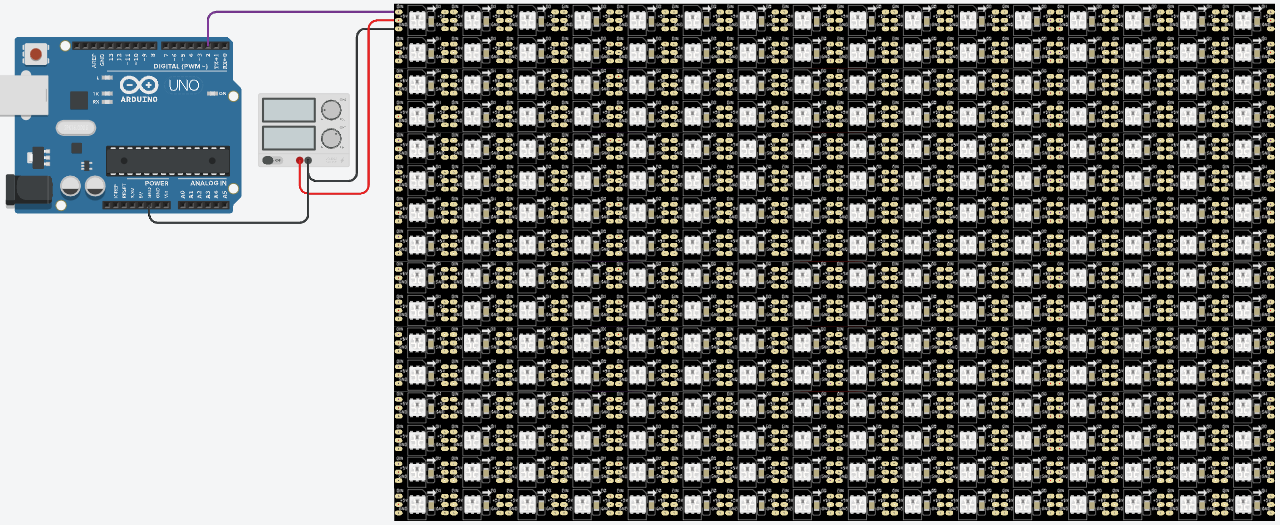
\includegraphics[width=12cm]{Images/leds.png}
    \centering
    \label{fig:leds}
    \end{figure}
    \vspace{0.5cm}
    
\section{Problemas Presentados}
\label{problemas}
    \begin{flushleft}
     \subsection{23/09}
     En este día, luego de plantear el código en QT, nos encontramos con la siguientes problematicas:
    \end{flushleft}
    
    \begin{flushleft}
    \subsubsection{Muestreos}
    Hasta el momento no hemos evaluado la técnica necesaria para realizar un submuestreo o sobremuestro según la imagen elegida, como su vez no hemos implementado la carga respectiva de la imagen.  
    \end{flushleft}
    
    \begin{flushleft}
    \subsubsection{Retorno de informacion}
    Para esta parte del programa, aún no tenemos muy claro como vamos a entregar la información requerida por Tinkercad de tal manera que se adapte a la representación de la matriz.  
    \end{flushleft}
    
    \begin{flushleft}
     \subsection{24/09}
     En este día realizamos la parte más sencilla del código que es sacar los datos de la imagen original, nos topamos con el problema de que no podíamos introducir todos los datos en una sola matriz, puesto que en algunos casos hay demasiada información, por lo que decidimos separar los datos en 3 arreglos, uno para los rojos, otro para los verdes y el último para los azules.
    \end{flushleft}
    
    \begin{flushleft}
     \subsection{25/09}
     En este día se hizo la mayor parte del programa de QT, debido a esto se nos impusieron varios predicamentos, entre ellos el tratamiento en matrices, esto debido a que en algunos casos una matriz tridimensional contenía demasiada información, por lo tanto nos vimos en la necesidad de repartir la información en distintas matrices bidimensionales; Otro problema que detectamos fue la fusión de colores, a pesar de no haber hecho aun los algoritmos de submuestreo y sobremuestreo, haciendo las pruebas de representar una imagen que ya contaba con las dimensiones de nuestra matriz de leds nos dimos cuenta de que en algunos casos los colores podían llegar a verse distorsionados, sin embargo debido a la información brindada por el profesor determinamos que era algo común y correcto que ocurra en algunos procesos de redimensionamiento de imágenes.
    \end{flushleft}

    
\section{Manual de Uso Rápido}
\label{manual}
    \begin{flushleft}
        
    \end{flushleft}

\vfill
\bibliographystyle{IEEEtran}


\end{document}
